\chapter{\statusgreen Related Work}
\label{chap:literature}

% \todoAWinline{There are a few general comments I have which run across the whole thing:
% 1) What exactly is propaganda, and what distinguishes it from persuasion? I think it would be helpful if you could clarify what you mean by each of the concepts, and check through your work to make sure you are using them consistently.
% 2) It would clarify things a lot if you could lay out your definitions properly. Rather than have them in-line as at the moment, choose a quotation environment and use that (I’ve flagged up several cases, but in case I’ve missed any).
% % 3) “Truthiness” doesn’t mean “the degree to which something is true”: it’s a satirical term. Do a search on your use of the word, and replace with either “accuracy” or “truthfulness” (or equivalent) depending on what it is you want to say.
% 4) There are several points where you make quite substantial claims without any evidential basis for them. Do make sure you always have evidence for your claims, either a citation or something else (sometimes it might be an experimental result, or a solid argument).}

In this chapter, we present the state of the art for the different research areas that are covered in the next chapters. Each of the sections is related to one of the Research Questions presented in Section~\ref{sec:intro_rqs}.

We start from the literature targeted to analysing similar articles (Section~\ref{sec:lit_relationships}), which considers relationships and similarities between different documents.
Then we move to the literature about persuasion detection, especially focusing on sentiment and propaganda detection (Section~\ref{sec:lit_persuasion}).
Next, we describe the literature about political leaning, illustrating the definitions and the approaches for the automatic classification (Section~\ref{sec:lit_leaning}).
And finally, we present the works on topic recognition, giving an overview of the existing approaches (Section~\ref{sec:lit_topics}).
After this overview of each of the areas covered, we present some additional related phenomena (Section~\ref{sec:lit_related}).

Subsequently, we discuss the limitations of not considering these research areas together, and the potential benefits of performing comparative analysis across dimensions (Section~\ref{sec:lit_discussion}).
To conclude, we present the scope of this work in Section~\ref{sec:lit_scope}.


% Similarity and parallel news

% \gls{propaganda}

% - Propaganda and misinformation

% \Gls{political-leaning}: definitions/classification

% topics

\section{\statusgreen Similarity between articles}
\label{sec:lit_relationships}

Our starting point is the literature that aims to analyse multiple versions of the same story, across different news sources.
From the enormous multitude of articles that get published every day, several datasets and resources of parallel news reports have been built (described in~\ref{ssec:lit_relationships_parallel}).
We are interested in works that explore what changes between similar articles, and the literature which defines and deals with different tasks (\ref{ssec:lit_relationships_tasks}). In particular, we focus on corroboration and omission detection (\ref{ssec:lit_relationships_corr_omiss}).

\subsection{\statusgreen Parallel News Reports}
\label{ssec:lit_relationships_parallel}

To talk about similarity between news articles, we first need to introduce the concept of \emph{parallel news reports}.
%
Parallel news reports are a specific type of \emph{parallel corpus}, a term that is frequently used when multiple languages are involved.
These resources, such as the OPUS dataset~\citep{tiedemann2012parallel}, are useful for applications in computational linguistics, translation studies and cross-linguistic corpus studies~\citep{brown1991aligning,ramesh2022samanantar,ziemski2016united,kunchukuttan2017iit,banon2020paracrawl}.

We take the use of this term in a monolingual setting, where each document contains a certain number of variations from the others, but still covers the same main events.
This specific interpretation is considered in works that perform sentence-level paraphrase extraction~\citep{dolan2004unsupervised,zhang2013harvesting}.
More specifically in the news media environment, several datasets and tools have been developed with the aim of exposing the users to several points of view~\citep{bozdag2015breaking}, in order to break the filter bubble~\citep{pariser2011filter}
%\todoAW{use eco chamber?}\todomargin{ better filter bubble https://medium.com/@nicklum/the-surprising-difference-between-filter-bubble-and-echo-chamber-b909ef2542cc}
that is built around them.

Some resources just group together news articles that are related, commonly known as news aggregators.
One example is Google News with the feature \emph{Full Coverage},\footnote{\url{https://blog.google/products/news/new-google-news-ai-meets-human-intelligence/}} that presents a collection of articles for each headline.
There are also resources that try to bring together opposing points of view, such as AllSides Headline Roundup,\footnote{\url{https://www.allsides.com/headline-roundups}} or research works that try to provide a similar result~\citep{trampuvs2015diversinews,park2009newscube}.


% \citet{bountouridis2018explaining}

Some of these resources are hand-curated while others are algorithmically synthesised. In the hand-curated groups (e.g., AllSides), there are usually domain experts or editors who manually put together news articles that share the same events and details. With AllSides, the editors select the articles from selected news sources to ensure that different sides of the story are presented.
Instead, with algorithmic resources (e.g., Google News Full Coverage), there is an automated approach that, based on clustering algorithms, creates groups of articles that cover the same story~\citep{marutho2018determination,alelyani2018feature,karimi2018news}.

\subsection{\statusgreen Common Tasks}
\label{ssec:lit_relationships_tasks}

With this availability of resources, specifically in the news domain but also more generally, the computational linguistics community has addressed several tasks.

First of all, we need to mention the \textit{semantic similarity} task.
Semantic similarity is defined as the likeness of meaning or semantic content as opposed to lexical similarity, which instead relies more on the exact terms matching~\citep{harispe2015semantic}.
The research community has created different benchmarks to evaluate models on their ability to capture the semantic similarity~\citep{conneau-kiela-2018-senteval,chandrasekaran2021evolution}.
As for what characterises the models, we have had an evolution over the last years, starting from the first generations of word embeddings~\citep{pennington2014glove,mikolov2013efficient}, up to the recent family of transformer-like models~\citep{devlin2018bert,cer2018universal,yang2019xlnet,reimers2019sentence}.

We then find another task that exploits similar ideas: \emph{finding related claims}~\citep{almeida2020text}.
This task is extremely useful for works that try to estimate the accuracy of claims, by looking for similar claims that have already been verified or refuted.
The literature uses this task as the first step in automated fact-checking~\citep{nakov2021automated,guo2022survey}.
This task is particularly challenging because small changes (e.g., a number reported or a negation) can drastically change the accuracy of a sentence.


% Suggest items to read (recommender systems)
Another task that relies on semantic similarity, is the \emph{recommendation of content} (e.g., news articles) that is similar to a given reference.
This opens the immense field of recommender systems~\citep{tintarev2006similarity,karimi2018news,feng2020news}, where there may be more than one objective function to satisfy.
Besides semantic similarity, the alignment with the point of view of the reader is important (but needs to be limited to avoid the filter-bubble effect)~\citep{lunardi2020metric,nguyen2014exploring,lunardi2019representing}.
For example, some approaches additionally consider the serendipity of recommendations as a secondary objective function~\citep{ziarani2021serendipity,abdollahpouri2021toward,raza2022news}.

Lastly, we can also consider as related the \emph{plagiarism detection} task.
In this task, the goal is to spot fragments of text that have been copied from others, without reference or with a certain proportion~\citep{stein2006near,alzahrani2010fuzzy,arabi2022improving}.
This is a research area that is particularly relevant and challenging nowadays given the incredible rise of generative models~\citep{openai2023gpt4}.
In recent months, the generation and detection of plagiarism have drastically changed, shifting from more literal matching to more advanced and less interpretable techniques.\footnote{e.g., \url{https://gptzero.me/} and \url{https://www.zerogpt.com/}}
%with tools that detect generated contents


\subsection{\statusgreen Corroboration and Omission Detection}
\label{ssec:lit_relationships_corr_omiss}

In addition to the tasks mentioned in the previous paragraphs,
\textit{corroboration and omission}
is another task identified by the computational linguistic community.
With this regard, our work focuses mostly on the investigation of corroboration and omissions
across multiple sources.
This task focuses on comparing and contrasting similar articles, to find which parts are in common and which ones are omitted~\citep{ehrhardt2021omission,bountouridis2018explaining,ko2023claimdiff}.
By analysing multiple news articles it becomes possible to understand the inter-relationships between multiple points of view.

For example, \citet{bountouridis2018explaining} extracts points of information (sentences) from articles, and cross-compares them across groups of related articles. In this way, it is possible to detect which details are corroborated in multiple sources and which ones are omitted.
Then the authors count the omissions and corroboration for each news source, and build an aggregated metric that is defined as the count of corroborations minus the count of omissions.
The rationale is that corroborating a detail with external sources indicates that the detail is more likely to be true.
Instead, if a news source omits a detail that other sources mention, it is considered as a negative indication.
Therefore, the more corroboration and the fewer omissions a news source contains, the more this metric is high.
The approach is validated by showing a positive correlation between these indicators and the values of credibility retrieved from Media Bias/Fact Check (MBFC).\footnote{\url{https://mediabiasfactcheck.com/}}
The scores of credibility of MBFC come from a computation derived from manually labelled features (e.g., factual reporting, bias).\footnote{\url{https://mediabiasfactcheck.com/methodology/}}

\subsection{\statusgreen Limitations}
% What is missing?

% Fine-grained study of the terms that change $\rightarrow$ our goal to expand
From these works on corroboration and omission detection, a limitation is that the analysis is performed only considering sentences but not the single words involved.
Once the related sentences are identified across articles, it would be very useful to analyse the slight variations in terms.
For example, it could be possible to identify terms that are unique and terms that instead are used across multiple sources. By bringing this analysis to the word level, we can be more specific about the variations and the commonalities between articles.
We will expand on this in Chapter~\ref{chap:common_ground_search}, where we address this limitation together with other limitations (e.g., semantic similarity models used, more resistant to term changes).

% What the term choice may mean (persuasion) $\rightarrow$ using literature on persuasion, considering multiple research areas together 
The next big limitation we find is that these publications often stop at the analysis of similarities, and do not study what these changes involve.
For this reason, in our work we also explore other related dimensions, such as persuasion.
Our aim is to see how the variations between multiple articles (specific term choices) cause changes in detected persuasion. In other words, what is the effect of using one term instead of a synonym that may carry an additional load?


% From the existing literature, we find that there are certain limitations that come from only analysing similarity
This type of limitation can be overcome only with a study that involves multiple factors at the same time, like a comparative analysis.

\section{\statusgreen Persuasion Detection}
\label{sec:lit_persuasion}

The next research area that we are touching in our work is \emph{persuasion detection}.
We are interested in getting an understanding of what words convey, beyond the simple expression of content.
Therefore, we want to have an additional study of what specific choices (terms, details, order of presentation) may convey.

% Before describing the literature, we need here to present our motivation for introducing this research topic. 


Contextualising in the current attention economy~\citep{davenport2001attention}, recent literature sees a rise in the race for attention also in news articles, with the emergence of clickbaitness and language that needs to be increasingly captivating~\citep{bazaco2019clickbait,davenport2001attention}.
With the enormous amount of news sources and news articles covering the same events, it is very important for news sources to compete for the clicks and reads of the consumers.

\citet{gass2018persuasion} defines persuasion as a method to ``influence a person's beliefs, attitudes, intentions, motivations, or behaviours".
We see several related concepts in the literature that can be considered as forms of persuasion. We select to explore two of them:
\begin{itemize}
    \item appeal to emotion / sentiment: use of emotional language to convey strong emotions to the reader~\citep{ginosar2019patriotic}; % loaded language instead?
    \item \gls{propaganda}:  information, ideas, opinions, or images, often only giving one part of an argument, that are broadcast, published, or in some other way spread with the intention of influencing people's opinions.\footnote{\url{https://dictionary.cambridge.org/dictionary/english/propaganda}}.
          The signature feature of propaganda is that it employs ``intentionally or unintentionally, flawed ideologies to cut off rational deliberation and discussion"~\citep{stanley2015propaganda}. % to indoctrinate a population towards an individual or a particular agenda
          % \item \gls{populism}: political ideas and activities that are intended to get the support of ordinary people by giving them what they want;\footnote{\url{https://dictionary.cambridge.org/dictionary/english/populism}}
          % \item coercion: use of force to persuade someone to do something that they are unwilling to do.\footnote{\url{https://dictionary.cambridge.org/dictionary/english/coercion}} % aggressive threats and the provocation of fear and/or shame to influence a person's behavior.
\end{itemize}
% \todoAW{Put in specific citations for these two cases.}

% Across these multiple forms, we explore in a more detailed way the first two: sentiment and propaganda.
Persuasion is linked with sentiment because of its goal to influence the emotional response~\citep{gatti2014sentiment,rocklage2018persuasion,petty2015emotion,desteno2004discrete}.
Instead, the relationship with propaganda comes from the inherent goal of propaganda to influence the public's view about an idea or a group~\citep{bernays,jowett2018propaganda}.

We dedicate the following two subsections to sentiment and propaganda detection respectively.

\subsection{\statusgreen Sentiment Analysis}
\label{sec:lit_sentiment}


Sentiment analysis is the computational treatment of opinions, sentiments and subjectivity of text~\citep{medhat2014sentiment}.
Several surveys have been published in the recent years~\citep{liu2010sentiment,medhat2014sentiment,wankhade2022survey}, and we rely on them to examine the tasks and techniques available.


% liu2010sentiment,medhat2014sentiment,wankhade2022survey : surveys

The first broad distinction that we need to make, is the granularity of the analysis.
Starting from the widest, we have \emph{document-level} classification, which means assigning to a whole document a single output.
Then, other approaches define the \emph{sentence-level} classification, which instead provides for each sentence an output. In this way, it is possible to analyse the evolution of the sentiment across a document, and get more detailed information.
The more detailed analyses provide \emph{aspect-level} classification~\citep{zhang2022survey}. In this case, we get an analysis of each aspect mentioned in the document. An aspect can be an entity or even a feature of an object (e.g., colour, shape) and in this way, the outputs are related to individual words or noun phrases.

The second distinction is based on the techniques used for the analysis. There are several techniques that range from simple dictionary-based to advanced deep-learning techniques.
The ones that have a longer history are the family of \emph{lexicon-based} models~\citep{taboada2011lexicon}. Being the simplest and most intuitive, there are many of them that are still very popular today. Even new models belonging to this family keep being developed, as it is a very powerful technique.
In this family, there are two subtypes: dictionary-based and corpus-based.
% https://www.sciencedirect.com/science/article/pii/S2090447914000550
Dictionary-based models depend on sentiment-carrying words that are used as seeds, and then search the dictionary for their synonyms and antonyms. In this way, large lists of words together with their sentiment are built~\citep{okango2022dictionary,hardeniya2016dictionary}.
Corpus-based models also start with seed terms, but then do the expansion with a corpus looking for synonyms, using statistical or semantic methods~\citep{darwich2019corpus,rice2021corpus}.

% They are built around a lexicon where each word has a specific score, and some combination rules. But we do not exclude tools that work with a different, more complex approach. It is only required from them to give a score specific to the individual words. 

From this family of approaches, we also have very popular tools that can be used freely, such as Sentistrength,\footnote{\url{http://sentistrength.wlv.ac.uk/}} Vader\footnote{\url{https://github.com/cjhutto/vaderSentiment}} and TextBlob.\footnote{\url{ https://textblob.readthedocs.io/}}


Instead, more advanced models are based on machine learning (mostly supervised, but also some unsupervised).
In the supervised approaches, we find examples of decision trees, Support Vector Machine, rule-based classifiers, Naive Bayes, Bayesian Networks, and Maximum Entropy approaches~\citep{zharmagambetov2015sentiment,bayhaqy2018sentiment,fitri2019sentiment,rathi2018sentiment,xie2019improved}.
The more recent ones rely on Deep-Learning models~\citep{zhang2018deep}, where there are multiple combinations considering:
\begin{itemize}
    \item document encoding: Bag of Words~\citep{moraes2013document,zhai2016semisupervised}, word embeddings~\citep{tang2015document,chen2016neural}, dense document vectors~\citep{le2014distributed}
    \item network architectures: feed-forward~\citep{duncan2015neural}, autoencoders~\citep{zhai2016semisupervised,wu2019semi}, CNN~\citep{jianqiang2018deep,sun2019aspect}, recurrent~\citep{chen2017recurrent,xu2016cached}, recursive~\citep{wang2016recursive,nguyen2015phrasernn}, memory networks~\citep{li2017end,lv2021aspect}
    \item attention mechanism: no attention, hierarchical~\citep{zhou2016attention} %, sequence, alignment
\end{itemize}



% Techniques of detection: (medhat2014sentiment)
% - lexicon-based
%   - dictionary-based
%   - corpus-based
%     - statistical
%     - semantic
% - ML-based
%   - supervised
%     - decision tree classifiers
%     - linear classifiers (SVM/Neural Networks)
%     - rule-based classifiers
%     - probabilistic classifiers (Naive Bayes, Bayesian Network, Maximum Entropy)
%     - Deep Learning (zhang2018deep survey):
%       - Document-Level classification
%         - Document representation: BoW, word embeddings, dense document vector
%         - Neural Network Model: Feedforward Neural Network, Autoencoder, CNN, Recurrent/LSTM/GRU, Memory Network
%         - Attention: No, Hierarchical, 
%       - Sentence-Level Classification
%         - Same as Document-level
%         - Adding: parse trees, opinion lexicons, and part-of-speech tags
%         - CNN/RNN: semantic and syntactic information from word embeddings
%       - Aspect-based Classification: Context, Target Representation, Sentiment Context (done with attention)
%   - unsupervised
%     - game theory
%     - based on sentiment clustering
%     - generative-model based: asking GPT-similar models, context of classification

% zhang2018deep : deep learning for sentiment analysis
% godbole2007large : large scale sentiment analysis

From this large group of publication and approaches, the solutions are less democratised, which means that it is usually very hard to reproduce the models and results, because of non-shared code-bases, datasets and parameters.
This means that there are less publicly available tools that perform this type of analysis.
One of the few exceptions is Stanford CoreNLP which is based on a Recurrent Neural Network~\citep{socher2013recursive} that accounts for the sequence but also for the dependency tree of the sentence (in other words, discovering the combination rules autonomously). It is based on a dataset that links sentiment scores to a dependency tree (Sentiment Treebank\footnote{\url{https://nlp.stanford.edu/sentiment/treebank.html}}).

% If at first glance, the advanced deep learning models may seem more reliable,\todoAW{You've not said anything about their performance, so I don't know whether they seem more reliable or not.} we find that the most robust and common methods are the simpler ones.
Given the recent trend of using deep learning ubiquitously, we may be persuaded that it is better to use big and complex models.
However, we have recent examples of lexicon-based approaches~\citep{okango2022dictionary,mitra2020sentiment}, as a proof that it is a technique very powerful still today.
For complex models instead, especially if in combination with aspect-based detection, we see that the status is yet in an exploratory phase, without major public tools made available ``off the shelf".

\subsection{\statusgreen Propaganda}
\label{sec:lit_propaganda}

Moving instead to \emph{propaganda}, we can start with some definitions.
According to~\citet{jowett2012propaganda}, ``propaganda  is  a  form  of  communication  that  attempts  to  achieve a  response  that  furthers  the  desired  intent  of  the  propagandist". This is slightly different from persuasion, which instead is ``interactive and attempts to satisfy the needs of both persuaded and persuaded"~\citep{jowett2018propaganda}.
% \todoAW{I'm finding both your definitions of propaganda and persuasion to be a bit woolly.
% Also: do you have a citation for this definition of persuasion?}
%A  model  of  propaganda  depicts  how  elements of  informative  and  persuasive  communication  may  be  incorporated into  propagandistic  communication,  thus  distinguishing  propaganda as  a  specific  class  of  communication.  References  are  made  to  past theories  of  rhetoric  that  indicate  propaganda  has  had  few  systematic theoretical  treatments  prior  to  the  20th  century.  Public  opinion  and behavioral change can be affected by propaganda.
% The terms propaganda and persuasion have been used interchangeably in the literature on propaganda, as well as in everyday speech. Propaganda employs persuasive strategies, but it differs from persuasion in purpose.





% TODO propaganda definition in different fields.

% First of all, let us start with a definition of propaganda.
We can then consider the definition from the Cambridge Dictionary, which defines propaganda as the use of language ``with the intention of influencing people's opinions".\footnote{\url{https://dictionary.cambridge.org/dictionary/english/propaganda}}
It has many points in common with argumentation and rhetorics and is usually associated with deceiving techniques, partial point of views, logical fallacies.
In his book on propaganda, Edward Bernays defines it as a ``consistent, enduring effort to create or shape events to influence the relations of the public to an enterprise, idea or group"~\citep{bernays}.

Propaganda possesses unique characteristics that go beyond its intention to persuade. It typically targets a significant audience, promotes the agenda of a particular group, and employs flawed reasoning and/or emotional appeals~\citep{miller1939techniques}.

Injecting propaganda into the political narrative is an old and common tactic to influence opinions and push certain ideologies or agendas.
Propaganda is very related to the agenda-setting theory \citep{Cohen_1964,mccombs1972agenda}, which describes the ability of news media to influence the importance placed on the topics of the public agenda.

It has become very relevant, especially in recent years, affecting the public discourse in more than 80 countries across the globe~\citep{bradshaw2021industrialized}.
It is not a recent phenomenon by itself, but it received a boost in diffusion thanks to the advance of technology.
For this reason, many works talk about \emph{computational propaganda} which underlines the strong relationship with technology and computational approaches.

\citet{hassan2023} define computational propaganda as ``the assemblage of digital platforms, algorithms, surplus data, and automation to curate, disseminate, amplify,
and increase discoverability of purposefully misleading information across the information
environment".
In the framework described by~\citet{hassan2023}, the media has a central position in amplifying propaganda and influencing the audience.

Propaganda can more practically be defined as the usage of a set of techniques. These techniques vary from the usage of emotional language (e.g. loaded language, appeal to fear) to logical fallacies (bandwagon, red herring).
%
Over the next paragraphs, %we first give more theoretical background about the \emph{propaganda model}, which describes the way that propaganda acts on society.
%Afterwards, 
we give an oversight to the most common propaganda techniques.
To conclude, we present some works that try to detect propaganda at different granularities.

% \subsubsection{The Propaganda Model}

% According to the propaganda model, which was developed by~\citet{herman1988manufacturing}, corporate mass media functions based on propaganda and systemic biases. It explains how populations are manipulated, and how consent for economic, social, and political policies is manufactured through propaganda. Media structures that create inherent conflicts of interest (e.g. advertising, media concentration, government sourcing) act as propaganda for anti-democratic forces, according to the theory.
% The theory relies on five \emph{filters} that determine the type of news that is presented in the media:

% % the problem is X taken from phillips2007left https://www.projectcensored.org/wp-content/uploads/2010/05/LeftProgressiveMediaInsideth_PropagandaModel.pdf
% \begin{enumerate}
%     \item Ownership: since the mainstream media outlets are usually big conglomerates, there will be some bias toward their interests in the information presented. The problem is the concentrated private ownership.
%     \item Advertising: the news is only a ``filler" to post advertisements, and therefore it needs to align with the ``buying mood". The problem is the orientation to profit.
%     \item Sourcing: first-hand news comes mostly from officials and powerful sources, because it is not affordable to have reporters everywhere. The problem is the over-reliance on governmental and corporate sources for news.
%     \item Flak: negative responses to the media statements or programs, such as complaints and other actions that are performed by organizations and coalitions, to disagree or to discredit. The problem is the tendency to avoid offending the powerful.
%     \item Fear: anti-ideologies (e.g. anti-communism historically, anti-terrorism) that exploit public fear of groups that are potentially a threat. The problem is religiously following the mainstream ideas, and strongly opposing alternative beliefs.
% \end{enumerate}

% These five filters together set what is considered acceptable in the coverage of daily events~\citep{phillips2007left}. ``Newsworthy" criteria influences journalists and editors, and everything that diverges from the ``common sense" is self-disciplined and self-censored.

% While the model primarily draws from U.S. media, Chomsky and Herman assert that the theory can be extended to any nation with similar fundamental economic and organizational foundations, as outlined by the model, which contribute to the emergence of media prejudices. This viewpoint has garnered support from various scholars, and investigations into the media's propagandistic functions have subsequently been conducted and validated in Western Europe and Latin America~\citep{herman1996propaganda}.


\subsubsection{Propaganda Techniques}

If we look at more practical definitions of propaganda, we see that in the literature several works have addressed propaganda as a set of techniques~\citep{torok2015symbiotic,miller1939techniques,weston2018rulebook}. The recent work of~\citet{da2019fine} takes from these works and considers only the techniques that can be found in journalistic articles and that can be judged intrinsically without needing external evidence.

These techniques are:
\begin{enumerate}
    \item Loaded language: employing language with strong emotional connotations;
    \item Name calling or labelling: attaching to the object of propaganda labels that trigger a negative (fear, hate, undesirability) or positive (love, praise) reaction;
    \item Repetition: repeating something multiple times, to make it accepted;
    \item Exaggeration or minimisation: using excesses to make something more or less important;
    \item Doubt: questioning the credibility of someone/something;
    \item Appeal to fear/prejudice: attempting to create support for an idea by increasing fear towards an alternative;
    \item Flag-waving: justifying an action based on the undue connection to nationalism or patriotism;
    \item Causal oversimplification: assuming that there is a single, simple cause of an outcome;
    \item Slogans: using a short and striking or memorable phrase;
    \item Appeal to authority: asserting the accuracy of a claim with the only evidence that someone authoritative supports it;
    \item Black and white fallacy: considering no middle way between two extremes;
    \item Thought-terminating cliché: not allowing critical thought using generic words usually from ``folk wisdom";
    \item Whataboutism: charging the opponent with hypocrisy without disproving their argument;
    \item Reductio ad Hitlerum: oppose an idea by suggesting it is popular in a group hated by the audience;
    \item Red herring: diverting the attention with unrelated material of conversation;
    \item Bandwagon: exploiting the desire of most people to join the crowd or be on the winning side, and avoid winding up the losing side;
    \item Obfuscation, intentional vagueness, confusion: willingly using unclear words or concepts;
    \item Straw man: caricaturing an opponent's position and then attacking it.
\end{enumerate}


\subsubsection{Propaganda detection (computational)}
\label{ssec:lit_propaganda_detection}

Developing computational methods to detect the use of propaganda in text is very recent, and is primarily fuelled by the increased use of propaganda in misinformation dissemination~\citep{da2020survey}.

% related work not granular
Most related work is limited to binary detection of propaganda (i.e. propaganda exists/does not exist) in general (i.e. regardless of propaganda technique), using n-gram logistic regression and SVM methods~\citep{rashkin2017truth,barron2019proppy}. This is performed at the document level only, without insights on which technique is used and where it is used in the text.


Several datasets for document-level detection have been released during the last decade.
First of all, in the English language:
TSHP-17~\citep{rashkin2017truth} and
QPROP~\citep{alberto_barron_cedeno_2019_3271522}.
We start to observe replications and additional works in other languages: for example in Hindi~\citep{chaudhari2022h,chaudhari_deptii_2022_5828240}
and in Czech~\citep{baisa2019benchmark}.

\begin{figure}[!htb]
    \centering
    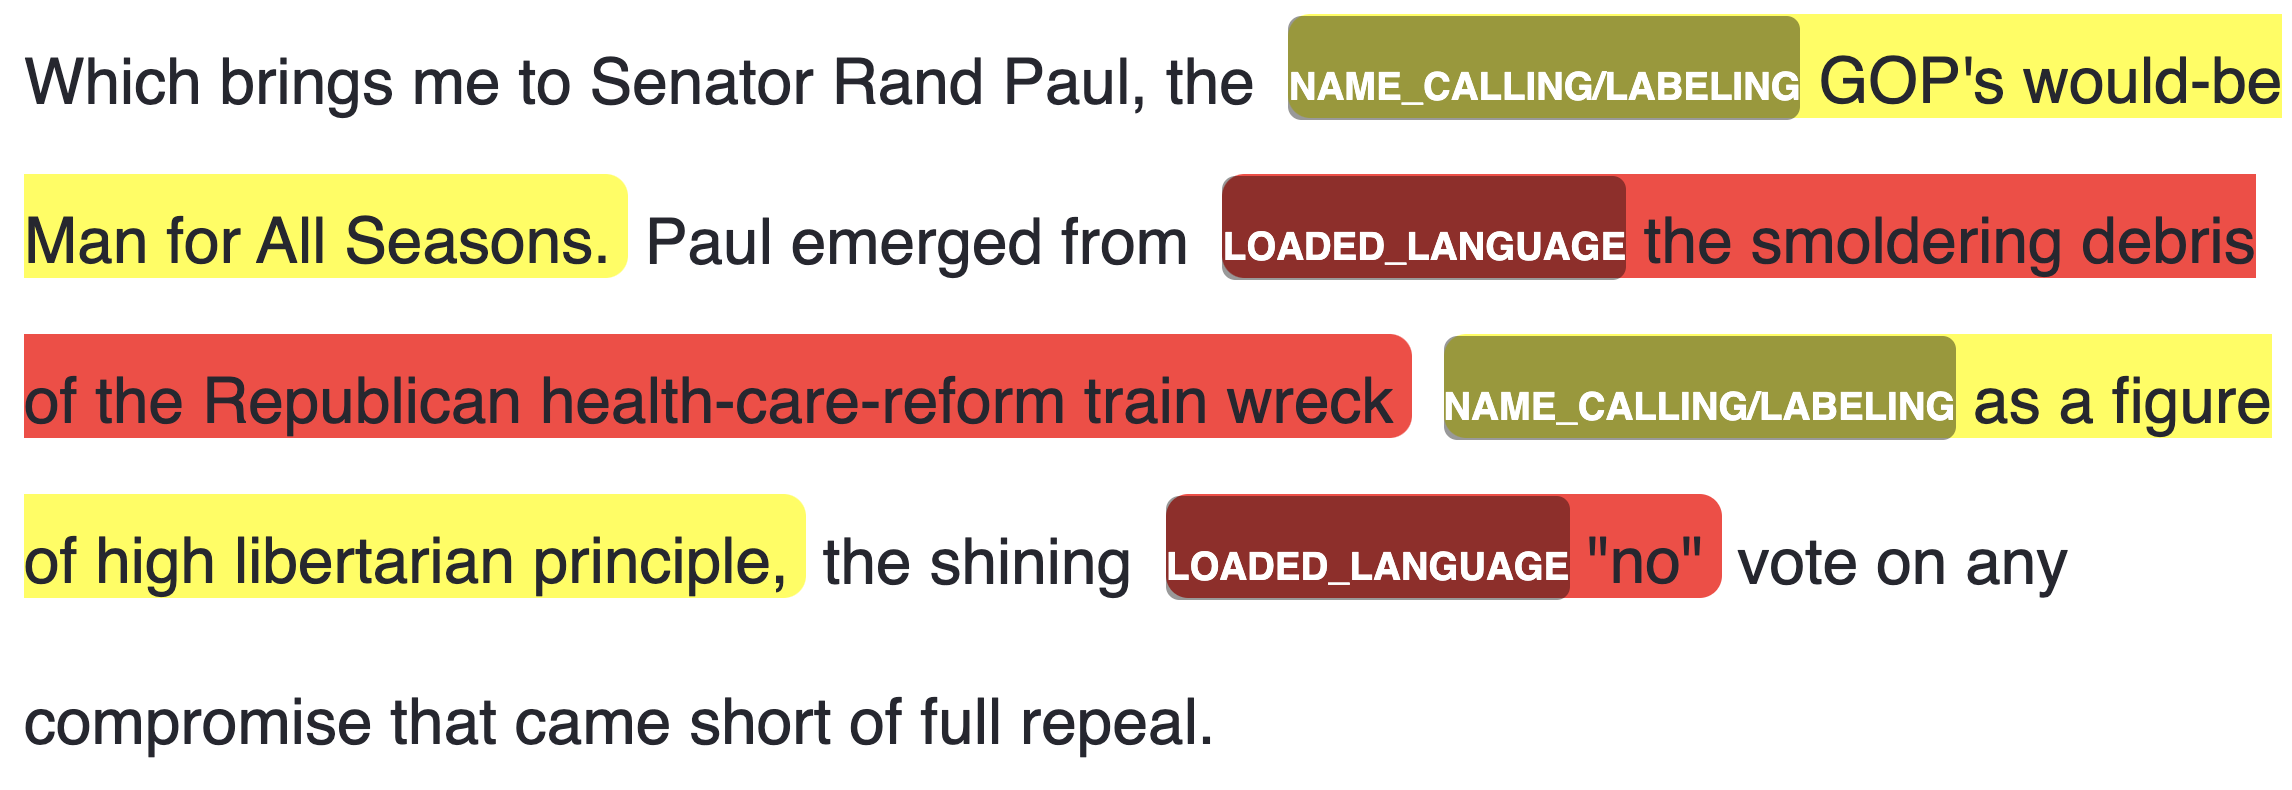
\includegraphics[width=\linewidth]{figures/propaganda_example_1_color.png}
    \caption{Detection of propaganda techniques using~\citet{baly2020we}.% the article comes from NationalReview, a source with Right-leaning bias.
    }
    \label{fig:propaganda_example_1}
\end{figure}

% granular
More recently, several works~\citep{da2019fine,yoosuf2019fine,vorakitphan2022protect} started doing a more fine-grained analysis, to identify fragments that contain propaganda, and the particular propaganda techniques used (Figure~\ref{fig:propaganda_example_1}).
These approaches use sequence models derived from BERT~\citep{devlin2018bert}, allowing us to have a much deeper insight into which parts of the text are propagandistic. Being the output of the models a sequence of tags, each word is labelled with the technique it belongs to (or none).
They all use the same dataset published in~\citet{da2019fine}, which enables different research groups to build models and progress on this task.


%On this, we have our hypothesis that \emph{we can recognise the political leaning of an article by using the features provided by the propaganda analysis}.
%The mixed analysis would allow to understand better why a certain article is classified as being left/right with respect to the black box BERT classifier.


%On the other side, we are considering the use of language that is targeted to push for a certain political view. There are many linguistic choices and techniques, along with how the narrative is structured, that are used to promote a specific viewpoint.
%Propaganda is defined as something that can be recognised by its persuasive function, sizeable target audience, the representation of a specific group’s agenda, and the use of faulty reasoning and/or emotional appeals~\citep{miller1939techniques}. The list of such techniques is very long\footnote{\url{https://en.wikipedia.org/wiki/Propaganda_techniques}}, and here we are considering the ones that have been analysed automatically by~\citet{da2019fine}. The propaganda is the most persuasive/loaded part of an article.
% \item sentiment usage: loaded language in the articles can reveal strong subjectivity against the mentioned entities. This relates to the subjective part of articles and we want to take this into consideration
% \item narrative/persuasion and other related analyses?



%For the propaganda analysis, we are focusing on the computational propaganda, defined as the propaganda that has been analysed by computational approaches. 
%The survey conducted by~\citet{da2020survey} displays the most important works, and also underlines the main limitation of current methods.
%The biggest limitation that we see, is that \emph{explainability is a desirable feature} but current approaches do not provide it.
%Most of the models only classify full articles as being propagandist or not~\citep{barron2019proppy,rashkin2017truth}, and this does not help to understand why.
%Therefore, another work focuses on fine-grained techniques~\citep{da2019fine}: every article analysed is annotated with labels coming from 18 different techniques, also indicating the spans affected by the techniques. So we can see where propaganda is inside an article and which specific techniques were used. Figure~\ref{fig:propaganda_example_1}

% TODO: The datasets for detection: article-level, fine-grained

\subsection{\statusgreen Limitations}

Sentiment detection has been researched extensively in the last twenty years~\citep{medhat2014sentiment}.
%for a long time.\todoAW{evidence/citation?}
However, the outputs of the analysis are usually limited to positive/negative.
Additionally, fine-grained analysis of aspect-based sentiment analysis cannot simply be used \emph{off the shelf} as pretrained models are typically not shared and the training requires large amounts of computational resources~\citep{brauwers2022survey}.
%do not demonstrate good generalisability strengths.
%\todoAW{evidence/citation?}
Nonetheless, there are tools available to perform document and sentence analysis, which can be used for word-level analysis by exploiting their lexicons.
%can allow a word-level analysis if used properly.\todoAW{Too informal.}
% For this reason, we deem sentiment analysis to be a good indicator of understanding the persuasion used in the articles.\todoAW{I don't see how this follows. Needs a bit more explanation.}

Propaganda detection, on the other hand, is relatively a young task.
While there are multiple datasets for document-level detection, only one dataset has been publicly shared for fine-grained (word+technique) analysis.
Therefore, there are potential limitations of the dataset and of the models trained with it.
There is, to the best of our knowledge, no study on the unbalance of this dataset. Models trained could be learning unwanted associations or not be comprehensive of propaganda with a context different from the examples contained in the training set.
% Applying propaganda detection ``in the wild" could cause both false positives and false negatives.\todoAW{That's true of all systems (including humans). The important question is probably what's to be done about it.}
Furthermore, the evaluation metrics of the existing models generally do not perform greatly.
For example, the work presented in~\citep{da2019fine} reports a span-level F1 of $22.5\%$.
This means that the task can be considered as difficult and with much room for improvements.
% provide lower-than-optimal values,\todoAW{"optimal" being what? 100\% accuracy? Equivalent to a human? etc?} denoting  this as a quite difficult task.
% explanation of lower than optimal
% From its publication paper~\citep{da2019fine}, we can see in table 6 and 7 that this model has been evaluated in two ways:
% \begin{itemize}
%     \item sentence-level: binary classification, whether the sentence contains propaganda or not. For this task the reported F1 is around $60\%$
%     \item span-level (full task): whether the corrects words have been identified with the correct technique or not, so accounting both for position/boundaries and for the label. For this task the reported F1 is slightly above $22.5\%$
% \end{itemize}
However, we use the outputs from this model to have an overview of the techniques used.
%\todoAW{Tighten up a bit... maybe comment on the SOTA to quantify "lower than optimal", and then use that to justify the claim for the difficulty of the task. Then be more precise about the value of the overview of the techniques "We give an overview of the techniques used, as this allows us to.../as this explains how..."}


We will use both sentiment and propaganda analysis in Chapter~\ref{chap:linguistic_persuasion} to see how we can combine this with the analysis of similarities across documents.
Furthermore, we will evaluate the limitations of the approaches available in our use case.

\subsection{\statusgreen Layers of Information}
\label{ssec:lit_layers_of_info}
We end this section with a reflection on persuasion techniques.
We described the detection of such techniques, but how intertwined are they with the contents and facts described in the news articles?
As the literature shows~\citep{jenkins2013thin,vanderwicken1995news,jang2023proximate}, text of articles can be seen as conveying two layers of information:
\begin{enumerate}
    \item the first layer, the most visible, is the layer of \emph{facts}: entities (what/who is mentioned) and actions (what happens), combined into events. This is usually called \emph{topic} made of \emph{topical words};
    \item a second layer of additional and subjective information: choice of terms to use, details to include and exclude, order of presentation, expression of opinion, subjective statements. All these means are used to convey a certain point of view, and therefore we use the umbrella term of \emph{persuasion} to include both sentiment and propaganda. This may be called \emph{anti-topical} component of the text.
          %\todoAW{I'm not clear what the difference is between propaganda and persuasion. And because of that, I'm generally unclear how you're using each term in the document.}
\end{enumerate}


% Talk here about different layers: 1 facts, 2 persuasion ( propaganda/argumentation/sentiment). Or in other terms: topical and non-topical elements.

These two layers can be more or less intertwined, and it can become more difficult to distinguish between them.
In the easiest cases, they can be identified on the linguistic surface of different words: some words in a sentence that belong to the \emph{facts} layer (e.g., a noun) accompanied by other words that belong to the \emph{persuasion} layer (e.g., an adjective).
In this case, it is conceptually easy to separate the two components in a text and say which word belongs to one or the other.
This is usually the case with adjectives, for example adding ``dreadful" next to a noun. We can recognise the adjective and separate it from the noun it accompanies.

But in many other cases, the two components can also coexist within the same word. A term may have been chosen both to communicate a certain concept (facts layer), but between many available terms, the author voluntarily or involuntarily picks one or another term that conveys a different opinion on the concept itself (persuasion layer).
For example, ``infanticide" compared to ``abortion" gives a very different connotation, and if we want to remove it we need to substitute the word with a more neutral synonym.
% \todoAW{For example?}

% e.g. name+adjective, where the name is the topical element while the adjective can express the opinion of the writer (commenting, denigrating, complimenting, subjective).
% Or they can also be expressed in the same word together: this is where word selection applies. For example, when the writer needs to find a word for communicating a certain concept ``?", they can choose whether to use X or Y. While these two words have the same underlying concept, they express it quite differently.

% Or also called: Topic model and Anti-topic model (expand on this, as discussed during the upgrade)

% Propaganda: Communication with the goal to persuade

Our hypothesis is that \emph{we can distinguish between the two layers}.
We will discuss this hypothesis in Chapter~\ref{chap:linguistic_persuasion}.


\section{\statusgreen Political Leaning}
\label{sec:lit_leaning}

In this section, we focus on the literature related to political leaning classification.
First, we give a definition of political leaning, and then we focus on the classification task and how it has been addressed by the literature.

\subsection{\statusgreen Political Leaning Definition}

Political Leaning is a term that is derived from Political Ideology~\citep{jost2009political}.
Political ideology is defined as a ``set of beliefs about the proper order of society and how it can be achieved"~\citep[p.~64]{erikson2015american}.

% From the multi-dimensional diversities\todoAW{What does this mean?} in political ideologies 
Political ideologies can be described with multiple independent dimensions (e.g., %goals in different fields such as economy, and methods as authoritarian vs libertarian
Collectivism vs Individualism, Progressivism vs Conservatism, Libertarianism vs Totalitarianism), but there is a historical tendency to consider only the Left-Right dimension~\citep{jost2009political}.
Although this simplification does not capture completely the complexity of determining one's political ideology, it is the most common way of describing political orientation.
Since only one dimension is considered, it is usually named as a political leaning or political spectrum.

% historical left and right

% https://www.dictionary.com/e/politics/political-spectrum/
% https://en.wikipedia.org/wiki/Political_spectrum
Historically, the usage of left and right originated during the 1789 French Revolution. The physical position of the politicians in the French National Assembly was sitting the revolutionaries on the left side, while the aristocracy-favouring was on the right.\footnote{\url{https://www.dictionary.com/e/politics/political-spectrum/}}
Therefore, the newspapers started using the terms to mention respectively the liberal with ``left" and the authoritarian with ``right".

% From originally only two labels, in 1857 we have the first appearance (on the Southern Trade magazine) of the term \emph{political spectrum} to describe the range of political opinions.\todoAW{Can you add a citation?}


% US and conservative vs liberal
% https://pleeps.org/en/wp-content/uploads/Political-Ideology-Its-Structure-Functions-and-Elective-Affinities.pdf (jost2009political)
The use of ``liberal" and ``conservative" as substitutes for ``left" and ``right" is becoming more prevalent in the United States and other countries.
This terminology effectively highlights the historical split between wanting change and desiring stability~\citep{jost2009political}.
These opposing desires emerge from long-standing discussions about proper levels of hierarchy, authority, and inequality~\citep{bobbio1996left}.
%\todoAW{I'm not sure where this is going...}


% % https://pleeps.org/en/wp-content/uploads/Political-Ideology-Its-Structure-Functions-and-Elective-Affinities.pdf (jost2009political)
% This formulation of the distinction between left and right is characterised by
% two different aspects~\citep{jost2018political}:
% \begin{itemize}
%     \item supporting vs opposing social change
%     \item rejecting vs accepting inequality
% \end{itemize}
% The most common terms that people from both left and right associate with the right are: “conservative,” “system maintenance,” “order,” “individualism,” “capitalism,” “nationalism,” and “fascism,” and they associated the left with “progressive,” “system change,” “equality,” “solidarity,” “protest,” “opposition,” “radical,” “socialism,” and “communism”~\citep[p.~213-14]{fuchs1990}.
% The two core components of the left-right dimension, attitudes towards change versus stability, and equality versus inequality, are connected due to historical factors, as Western societies have gradually become more egalitarian over the past few centuries in terms of human rights and liberties, economic distribution, and political power distribution.
% Equality has increased in some instances due to revolutionary events, which were frequently resisted or opposed by conservatives and those associated with the right~\citep{nosek2009politics,burke1790reflections}.



% automated paragraphs
Left-leaning ideologies are typically associated with progressive and socialist ideas, such as the belief in social equality, the importance of government intervention in economic matters, and the provision of public services.
Right-leaning ideologies, on the other hand, tend to prioritize individualism, capitalism, and free markets, with less emphasis on government intervention and regulation.

However, the specific meaning of left and right can vary across countries and political systems.
For instance, in some countries, left-wing political parties may advocate for more social welfare programs and nationalized industries, while in others, they may focus on issues such as civil liberties and human rights.
Similarly, right-wing parties may prioritize issues such as nationalism, religious conservatism, or economic liberalism, depending on the country's culture and political history.

Furthermore, the labels ``left" and ``right" can also be influenced by the particular issues and events of a given time period.
For example, in some countries, environmentalism and climate change have become important political issues that may cut across traditional left-right divides.
Similarly, issues such as immigration, trade, and national security may be more salient in certain countries than in others, shaping the way that people identify with different political ideologies.




% practical definition: view on issues


% Position of the left and right (wikipedia/allSides):

% https://www.allsides.com/media-bias/rate-your-bias
\begin{table}[ht]
    \centering
    \resizebox{\textwidth}{!}{
        \begin{tabular}{p{0.25\linewidth} | p{0.55\linewidth} | p{0.55\linewidth}}
            Topic         & Left                                                          & Right                                                                            \\ \hline
            % Social issues & \\
            Abortion      & rights of the mother, ability to have abortion                & rights of the fetus, limiting or stopping abortions                              \\ \hline
            Gay marriages & no difference with opposite-sex couples                       & sacred marriage between man and woman                                            \\ \hline
            Family        & expanded view on non-traditional families                     & not encouraging divorced, single, unmarried parents (accepting them may be fine) \\ \hline
            Taxes         & tax increases on the wealthy and more progressive tax systems & decrease taxes for everyone                                                      \\
            % Sex and Gender & accepting and empathetic culture & \\
            % Sexuality & free expression is a right & \\
        \end{tabular}
    }
    \caption{Example of Left and Right positions according to AllSides.}
    \label{tab:allsides_leaning_positions}
\end{table}

As a more practical and operable definition, we can define political leaning from the common positions that left and right have on issues such as economics, social policies, and governance.

Table~\ref{tab:allsides_leaning_positions} shows an example of how AllSides recaps the common positions about different issues, but the complete list is larger.\footnote{\url{https://www.allsides.com/media-bias/rate-your-bias}}
Perspectives on multiple topics are listed: social issues, economic issues, foreign policy, environment and energy, healthcare, education, social security, and welfare.
%\todoAW{I think there's too much here on left/right politics, but maybe there's no need to remove it. But I think I'd put a bit more in on AllSides, such as how it's curated, and that sort of thing.}




\subsection{\statusgreen Political Leaning Classification}
\label{ssec:lit_leaning_classification}


%First we present literature on political leaning prediction, then on propaganda detection, and how the two analyses could be connected. %with the possible points of contact and why the two analysis could benefit from an integration.

%\subsection{Political Leaning}
% Political leaning classification

Political leaning detection models have been produced for general media sources~\citep{budak} or for
specific political corpora such as congressional records~\citep{gentzkow}, political party websites~\citep{yan2017perils}, and political blogs~\citep{ahmed201}.
Others focused on inferring the political leaning of Twitter accounts~\citep{Cohen2013ClassifyingPO}, Facebook users~\citep{Bakshy1130}, politicians~\citep{thomas-etal-2006-get}, or political writers~\citep{iyyer-etal-2014-political}.

Various analysis methods were used in such studies, such as linguistic analysis \citep{gentzkow}, graph analysis \citep{chen2017opinion}, topic modelling \citep{ahmed201, Cohen2013ClassifyingPO}, support vector machines (SVM) \citep{Bakshy1130,thomas-etal-2006-get}, and neural networks \citep{iyyer-etal-2014-political,baly2020we}.


%often used supervised or unsupervised models applied to , or on opinion graph mining ~\citep{thomas-etal-2006-get}.

%gentzkow - linguistic analysis 
%yan2017perils - regression models and neural networks
%budak - supervised learning and crowdsourcing
%ahmed - topic models
%Cohen2013ClassifyingPO - SVM and topic models
%bakshy support vector machine 
%thomas - svm
%iyyer - NN
%chen - SVM, LDA

%Most models use supervised or unsupervised machine learning algorithms, trained using source annotations or crowdsourced articles annotations  

%underlined that most of the approaches do not generalise well across domains. 
%As~\citet{yan2017perils} underline, three different classifiers trained on different types of texts (domains: congressional records~\citep{gentzkow}, political websites, wiki) result in lack of cross-domain generalisability (classifier trained on different domain struggles to find correct label on another domain, and mixing the training data reduces performance confusing the models).

In~\citet{baly2020we}, authors used a BERT-based~\citep{devlin2018bert} model for predicting the political leaning of individual articles. The model takes as input the text of the article and produces one of three labels: Left/Centre/Right. The model is trained with a corpus from AllSides website,\footnote{\url{https://www.allsides.com}} which groups articles %with their political leaning 
according to the leaning of their source or of their author.


The main focus in~\citet{baly2020we} is to classify individual articles regardless of the source or author. This generalises better with unseen sources, and with cases where there is a difference between the political leaning of a particular article from that of its source.
% Authors found that 3.11\% of their 34737 articles from AllSides has a different leaning to the given to their sources (AllSides confirmed that this is due to using author-based leaning labels for some articles). 
This is a significant difference compared to approaches that only learn the media bias of the source~\citep{baly2020written,biessmann2016automating}.

To achieve this result, the authors use a specially crafted triplet loss~\citep{schroff2015facenet}, where the positive example shares the same political leaning but is published by different media, while the negative one has a different political leaning but is published by the same source. In this way, the encoder will encode more similarly the articles with the same leaning and different source.

Moving to the datasets, there are several resources available.
Most of them provide the annotation of the political leaning at the source level. In other words, the annotated data consists of lists of sources for each political leaning. This can be accompanied by a collection of articles with their full text, but there is no direct annotation of the leaning of the articles themselves.
Between the resources that list the political leaning of sources, we can mention Media Bias/Fact Check\footnote{\url{https://mediabiasfactcheck.com/}} and NELA-GT-2018~\citep{DVN/ULHLCB_2019}.
In addition, AllSides gives the label to the source level but sometimes also to the author level. This last resource is the origin of the dataset provided together with the paper from~\citet{baly2020we}.
%Authors found that 3.11\% of their 34737 articles from AllSides has a different leaning to that given to their sources (AllSides confirmed that this is due to using author-based leaning). 
%   \item source-level annotation: in most of the cases, the articles are annotated with the bias of the media outlet
%   \item author-level annotation: sometimes, the articles are annotated with the bias of the specific writer, which can be
% Similarly to \citet{baly2020we}, in this paper we also focus on classifying articles, regardless of their source and authorship. However, %unlike ~\citep{baly2020we}, 
% unlike previous work, we use propaganda features in the political learning prediction model.   

% - Problem: learning the source instead of the political leaning
%Main focus in~\citet{baly2020we} is to classify individual articles regardless of the source or author. This generalises better with unseen sources, and with cases were there is a difference between the political leaning of a particular article from that of its source. Authors found that 3.11\% of their 34737 articles from AllSides has a different leaning to the given to their sources (AllSides confirmed that this is due to using author-based leaning labels for some articles). 


%Other approaches focus on learning the media bias of a the source~\citep{baly2020written,biessmann2016automating}.
%This is based on the observation that in their dataset (collected from AllSides) there are some articles (1,080 individual articles, 3.11\% on a total of 34737) having a leaning different from their source leaning.

%To clarify this point, we personally asked to the AllSides team about this discrepancy between article-level bias and source bias, and we understood that there are two types of annotation:
%\begin{itemize}
%   \item source-level annotation: in most of the cases, the articles are annotated with the bias of the media outlet
%   \item author-level annotation: sometimes, the articles are annotated with the bias of the specific writer, which can be different from the media bias\footnote{\url{https://www.allsides.com/media-bias/media-bias-ratings\#ratings}}
%\end{itemize}

%Therefore the 3.11\% is due to the author-level annotation. We want to underline that in this way, the annotation of the political leaning is not specifically assigned to the single article but instead it is assigned to the author. It is still a "distant supervision" in some extent.

% - Problem: domain generalisation does not work
%Other works on political orientation prediction underlined that most of the approaches do not generalise well across domains. As~\citet{yan2017perils} underline, three different classifiers trained on different types of texts (domains: congressional records, media websites, wiki) result in lack of cross-domain generalisability (classifier trained on different domain struggles to find correct label on another domain, and mixing the training data reduces performance confusing the models).


% TODO: Is this really a consequence of the previous paragraph?
%Because of this lack of generalisability, 
%Other models focused on identifying political leaning using opinion graphs that represent how (positive/neutral/negative) the political leaning sees a set of extracted entities~\citep{chen2017opinion}. The prediction of the classifier, after extracting the entities in the text, compares the orientation towards the entities and picks the most similar side.
%The task of topical stance is also explored in other works in relationship to the political leaning of a whole news source~\citep{stefanov2020predicting}.
%A similar approach is described in~\citet{jiang2008political}, where instead of opinion the term used is subjectivities. The authors show how, by using the same model (Bag of Words) on the subjective sentences only, it is actually easier to classify political leaning. Furthermore, they mine Opinion Expressions which represent the orientation towards specific expressions (e.g., the liberal political leaning usually refers to ``democratic party'' using a positive subjectivity).
%These models rely on the fact that political leanings often have a stable view on some topics\footnote{\url{https://en.wikipedia.org/wiki/Right-wing_politics}}\footnote{\url{https://en.wikipedia.org/wiki/Left-wing_politics}}.








% Sentiment analysis

% Propaganda analysis

% Fine-grained

% AllSides and comparison of multiple sides, the summary contains some insights about the biggest differences between the political sides.

% Bias / political leaning classifier:
% - baly et al 2020: just based on text
% - we could help the models focusing on the layer of presentation/bias/propaganda instead of having the full text



% Two axes:
% - common/unique
% - objective/subjective/framing

% Different. The first one can be observed with similarity analysis. The second one with sentiment/propaganda/framing analysis.

% The left/center/right political leaning is mostly positioned on the common/unique axis.

% Hypothesis: the two axes are very much correlated. Looking at the framing axis can help to distinguish political bias.

% We try in the next sections to see if this is true.

\subsection{\statusgreen Limitations}

For political leaning, we found a large literature that
%the existing approaches are quite good at 
classifies the leaning of articles.
%\todoAW{Are they? Don't put statements like this in without quantifying them. How good are the existing approaches at classifying the leaning of articles? And where do you demonstrate it in the document?}
%
% would be nice to see relationship between leaning and persuasion
What we find slightly limiting, is that the existing works consider political leaning on its own. It could be very interesting to analyse the interaction between political leaning and persuasion, finding patterns between the two. This is where we aim to bring our contribution with this thesis.
We aim to understand which techniques change the most across the political spectrum, both in quantity and in terminology. At the current state of existing works, there is no insight into this.

%As a second limitation,\todoAW{It's not a limitation, it's a question. Either re-express the second part of the sentence as a limitation, or re-express the first part as a goal.} we question to what extent we could improve the political leaning classification of news articles by considering propaganda analysis.
Considering political leaning and propaganda computational studies jointly could bring improvements in the current state of the art in tasks such as political leaning classification. These models could try to use propaganda features to make better predictions.
Our \acrshort{rq}3 goes in this direction by hypothesising a relationship between the two dimensions.



\section{\statusgreen Topics}
\label{sec:lit_topics}

The last area of research that we cover in this thesis is the one related to topic analysis.
As for the other sections, we first present a more theoretical background and then we describe the main techniques used to identify topics.

% \citet{garimella2018quantifying,treuillier2022being} that state that some topics have more polarizing effects because they present higher or lower levels of controversy.

\subsection{\statusgreen Topic Definition}
\label{sec:lit_topics_def}

We can start with a definition from the Cambridge Dictionary, which defines topic as ``a subject that is discussed, written about, or studied".\footnote{\url{https://dictionary.cambridge.org/dictionary/english/topic}}

The analysis of the topic aims to understand what the text is about, and what it covers. We find several definitions in dictionaries, and each one of them slightly differs from the other.
This is true also for definitions from scientific literature, where we find quite significant differences in topic-related publications.
For instance, %~\citet{jo2007detecting} define topics as semantic units that can function as building blocks for discovering knowledge. For
~\citet{ding2011community}, views topics as document categories with various aspects, which can be specific to domains, applications, and contexts.

Practical definitions, like those rooted in topic modeling, view topics as groups of closely related words that share a certain probability of occurrence~\citep{blei2003latent,blei2006correlated,blei2012probabilistic}, or based on keywords \citep{erten2004exploring,decker2007detection}.

% What it is:
% - categories / groups 

Strictly related to news media, we have a practical definition that comes from IPTC (global standard body of the News Media) which has a specific standardisation for \emph{media topics}.
The media topics consist of a taxonomy where there is a hierarchy from course-level topics to more fine-grained ones.
The taxonomy is specific to news, and it defines 17 top-level topics, which are then expanded with different levels of detail.
The full hierarchy with all the labels can be seen online.\footnote{\url{https://www.iptc.org/std/NewsCodes/treeview/mediatopic/mediatopic-en-GB.html}}
IPTC also makes available an interactive TreeView where topics can be explored and expanded.\footnote{\url{https://show.newscodes.org/index.html?newscodes=medtop&lang=en-GB&startTo=Show}}
This taxonomy can be used as a conceptual method to annotate and compare topics uniformly.

% Definition IPTC
% IPTC media topics: hierarchical topics, defined by IPTC (global standard body of the News Media) with a topology.\footnote{\url{https://www.iptc.org/std/NewsCodes/treeview/mediatopic/mediatopic-en-GB.html}}
%     The topology is specific to news, and it defines 17 top-level topics, which are then expanded with different levels of detail. TextRazor provides this type of topic, as for the other ones, as a set of 5 for each input article with the relative probability. So for each one of the topics, we can understand where it is placed in the hierarchy and the parent topics.


% How it relates to concepts described in this thesis:
% - headlines, clusters
% - topic and anti-topic layers/words: refer to Chapter~\ref{ssec:lit_layers_of_info}

% We see across the literature several types of topics

\subsection{\statusgreen Computational Approaches}
\label{sec:lit_topics_computation}

Moving to the computational side, there exist many topic modelling methods~\citep{vayansky2020review,ramage2009topic,churchill2022evolution,kherwa2019topic}.
We can identify two main groups:
\begin{enumerate}
    \item unlabelled: frequency-based, that are mostly unsupervised. This group typically is made of clustering algorithms that, given a number of topics to produce, generate the output clusters. Therefore, they typically do not provide output labels. %We describe briefly the family of LDA approaches below, that belongs to this group.
    \item labelled: this group instead provides labelled topics in output, that are usually specified a priori (e.g., topology-based) or relate to entity types and custom patterns.
\end{enumerate}


% topic for fine-grained opinion analysis~\citep{stoyanov2008topic}


% Explain here different tools/methods that provide topics/entities

We describe in the following paragraphs some example approaches that belong to these two groups.


\subsubsection{Latent Dirichlet Allocation}

Belonging to the first group of methods of topic modelling, we have \acrfull{lda}.
%
% One of the most common methods to extract topics is to ``automatically detecting them" from the corpus.
% The idea is to learn from the data and by selecting a specific number of output topics, we get them.
%
% Topic identification is a method for identifying hidden subjects in enormous amounts of text1. It can help you find common themes or keywords that represent the main ideas of a document or a collection of documents. For example, if you have a set of news articles, you can use topic identification to find out what are the most discussed topics among them.
%
% One of the techniques for topic identification is called Latent Dirichlet Allocation (LDA)12. 
This is a statistical model that assumes that each document is composed of a mixture of topics, and each topic is composed of a distribution of words.
The approach uses a generative probabilistic model and Dirichlet distributions.
\acrshort{lda} can learn topics and words from the data without any prior knowledge or labels.
%LDA can be implemented using Python’s Gensim package1, which provides various tools for natural language processing.

% LDA is a type of topic modeling that uses a latent Dirichlet allocation approach12. 
% Topic modeling is a form of unsupervised learning that can be used for exploring unstructured text data by inferring the relationships that exist between the words in a set of documents23.

% LDA assumes that each document is composed of a mixture of topics, and each topic is composed of a distribution of words13. LDA can discover topics that are hidden (latent) in a set of text documents by inferring possible topics based on the words in the documents34.

% Another technique for topic identification is called bag-of-words2. It is a simple way to represent text data as a collection of words and their frequencies. Bag-of-words ignores the order and structure of sentences, but it can capture some basic information about the content and vocabulary of a document. Bag-of-words can be used with simple NLP models such as TF-IDF or Naive Bayes to identify topics from texts.

% Problem: difficult to extract labels
This method, like other unlabelled approaches, has a major drawback: it is difficult to extract topic labels.
%The outputs of the model are clusters of documents, and most important words for each of the clusters. But the process is not easy to have a label for the topic from this information. Usually, in the literature there is a step of manual revision of the clusters and the important words and then a manual labelling of the clusters.
%During this manual revision, it can emerge the problem that clusters look similar or related, and it may be necessary to join the clusters together or to modify the number of desired clusters and run the method again.\todoAW{from ``the outputs" onwards: Feels a bit clumsy, and not evidenced. Find a suitable citation, and use it to help rephrase.}
These models produce in output clusters of documents and the most important words for each of the clusters.
However, it is quite difficult to assign meaningful labels to the produced clusters, as the identified words usually overlap and may be quite diverse for a single cluster.
Therefore, there is usually need for a manual labelling step which may involve joining existing clusters together because they are similar.
Being this process not completely automatised, we prefer to use approaches that assign topic labels that are known beforehand.

% The problem of assigning labels: can we really tell what is different about the groups?

% Need to know beforehand how many topics we want in output.
The second big problem is that the number of output topics needs to be inserted as input parameter to the algorithm. This means that multiple runs are necessary and the study of this hyperparameter is something very critical.

Also other approaches that belong to the same group of topic modelling, have the same limitations even if they use more advanced features~\citep{wang2012nonnegative,landauer1998introduction,grootendorst2022bertopic}.


\subsubsection{Knowledge-based}

A different approach to topic modelling is instead taken by knowledge-based topic modelling.
%
This type of approach~\citep{chen2013leveraging,allahyari2017knowledge,xu2018hierarchical,ali2019transportation} relies on an external source of knowledge that can be a flat list of topics to align with, a taxonomy of topics, or a complete Knowledge Base containing entities and relationships.

With difference to the first group of methods, this family has two phases.
In the first phase, features are extracted from the documents (entities, term frequencies).
The second phase, missing in the first type of model, tries to align to the defined topics and estimate the probabilities of belonging to each of them.

With respect to the first group, we have less availability of such methods to the general public, as there is less standardisation of the topics (they change depending on the domain of application).
We see more commercial tools related to this group of approaches (e.g., TextRazor,\footnote{\url{https://www.textrazor.com/}} which can analyse topics with the taxonomies of IAB content and IPTC mediatopics).

% We have approaches that try to determine the topics without having external knowledge, and approaches that use instead an existing taxonomy/list of topics and try to map the input documents to them.


% DBPedia spotlight: entity annotation is not very good. It struggles to recognise all the entities in the articles (proof?) → DISCARDED
% BLINK (Facebook): huge (30GB models to fit on RAM), not running on my laptop. On server: no NVIDIA drivers (wants GPU) → DISCARDED
% Spacy-entity-linker https://github.com/egerber/spaCy-entity-linker/ . Not very widely used. → DISCARDED

% Then from entities, need ways to derive the topics by navigating knowledge bases (wikidata in most cases)

% \subsubsection{TextRazor}
% TextRazor: seems more accurate, industrial, FreeBase taxonomy. Each entity is annotated with wikidata id and a list of FreeBase types. Also provides topics and fine-grained topics

% benchmarks? check that it is better than other tools
% Regarding the validation of TextRazor, I am not aware of a benchmark done to check if it is better than other tools. It was suggested by Harith to use it, and I find that the data it provides is generally quite good (for topics and entities). But this is qualitative, I didn’t do a benchmark or looked up for benchmarks. The assumption was that it’s a commercial product and it should be good.
% some papers that claim to do benchmarks:
% http://giusepperizzo.github.io/publications/Rizzo\_Erp-LREC2014.pdf for the entities
% https://www.linkedin.com/pulse/google-nli-kill-market-linguistic-apis-review-yuri-kitin/ mentioning that TextRazor is useful because it links to Wikipedia/DBPedia

% TextRazor is the only one that provides already hierarchical topics, the other ones always give topics that are not hierarchical or can be made hierarchical with external knowledge (e.g. using DBPedia to navigate broader topics).

% What it provides


\subsection{\statusgreen Limitations}

With this section, we have seen several methods to extract and analyse topics.

We have on one side approaches that do not provide labels, and on the other side approaches that provide labels but are more commercial.
% commercial solutions, labels
Depending on the goals of topic analysis, the first group could be not very useful. For example, if we want to have hierarchical labelled topics, it is crucial that the topic analysis provides topic labels on its own.
In our case, we want to analyse how persuasion changes across topics, and having the labels is very important. Therefore, we do not want to apply the first type of topic modelling.

% Missing analysis of the links between topics and other dimensions (leaning and persuasion)
As main limitation of both types of approaches, the topic analysis is usually performed in isolation with respect to other dimensions.
Instead, we want to analyse topics together with persuasion, political leaning and similarities.
We see some works that do topic analysis with other factors (e.g., joint topic and opinion analysis in~\citet{stoyanov2008topic}), but not together with propaganda or political leaning.

\section{\statusgreen Related Phenomena}
\label{sec:lit_related}

In this section we cover other phenomena that are related but are outside the scope of this thesis.
We discuss them to acknowledge their existence and their relationship with our research.
% In the following subsections, we cover the relationship with misinformation and populism.
%, argumentation mining and defend the scope of this thesis: propaganda.

% But at the same time mention the relationship with them

\subsection{Misinformation}
\label{sec:lit_related_misinformation}

A very important area of research, that exploded in terms of publications in the recent years, is misinformation.
There have been huge waves of misinformation related to the recent events (e.g., elections, COVID) and the research community is actively trying to mitigate the spread by enabling faster recognition and verification of claims.

Misinformation is conceptually related to propaganda, using its techniques to make false information more likeable, shareable and assimilable.


For example, in~\citet{orrumachine} persuasiveness is observed to exist more in fake news outlets. As a key result, persuasive discursive repertoires appear more in fake news, while some other discursive repertoires that are less persuasive appear in more trustworthy news outlets.

Then we have also works that consider manipulation techniques closely related to propaganda and logical fallacies~\citep{roozenbeek2022countering}.
%Good evidence that making people aware is helpful, people can learn to recognise manipulation techniques (it worked on YouTube). The paper talks about manipulation, but the techniques overlap with propaganda and logical fallacies. Also shifts the goal from recognising True/False to recognising manipulation. Work from Psychology.
As another example, the work of~\citet{romain2022misinformation} relates the two concepts, considering persuasive writing strategies for misinformation detection.
Also in our previous work on credibility measures~\citep{mensio2019news}, %TTO2019 comparison of different credibility measures, and 
we saw that propagandistic sources are usually considered as part of misinformation, as the Media Bias/Fact Check data conceptually places propaganda inside the ``questionable news sources / fake news".

% This relationship between
% Rating news sources in different aspects
% TODO: here talk about all the tools/websites that rank news sources or score them with respect to misinformation/propaganda/bias/leaning

% CONCLUSION:
As general observation, misinformation typically uses propaganda, but the relationship is not bidirectional. In this work we do not investigate on the accuracy of the news, but we focus on the linguistic means of persuasion (propaganda).
By doing so, our results should be more general, and if needed can be applied to misinformation (with appropriate adaptations).

\subsection{Propaganda and Populism}
\label{sec:lit_related_populism}
% \todoAW{You want some evidence/citation to demonstrate that this is an actual area of research}
% Relationship between propaganda and populism:
% ~\citep{oates2021rewired,tumber2021routledge,pasquino2008populism}
%https://ebrary.net/177441/sociology/the_routledge_companion_to_media_disinformation_and_populism
% they are very strictly linked.
% http://www.ask-force.org/web/Fundamentalists/Pasquino-Populism-and-Democrady-2005.pdf 

% % concepts
On the conceptual level, propaganda and populism are two distinct concepts. The first describes more the persuasion mean used to push for an agenda, while the second one is typically used more in association with the actor that wants to push the agenda. Populism is ``a type of politics that claims to represent the opinions and wishes of ordinary people".\footnote{\url{https://www.oxfordlearnersdictionaries.com/definition/english/populism}}
To be on the side of ordinary people, it uses propaganda as a mean. So a populistic \emph{actor} uses propaganda \emph{techniques}. Therefore, even with their distinction, they are related.
% We need them to be related to demonstrate that propaganda exists across all political leanings.


Literature presents propaganda and populism frequently together~\citep{oates2021rewired,tumber2021routledge,pasquino2008populism}.
\citet{oates2021rewired} expresses the
concept of \emph{rewired propaganda} to analyse the interplay of propaganda and populism. Online information, while making citizens more informed, is overshadowed by the internet's ability to spread false information through populist propaganda.
The idea of ``rewired propaganda" is proposed as a way to explain a method of communication that uses false information and campaign strategies, especially evident in how both traditional and social media worked during the 2016 US elections.
When populism takes over from ideology-based politics, like in the 2016 US elections, rewired propaganda becomes as influential in democracies as it has been in non-free countries like Russia.

While populism detection is outside of the scope of this thesis, we use the relationship between populism and propaganda in Appendix~\ref{app:prop_and_populism} to support our analysis of the imbalance of propaganda datasets.


% \subsection{Opinion and Subjectivity and Manipulation?}


\section{\statusgreen Discussion}
\label{sec:lit_discussion}

After having presented the different research areas that we relate with, we present here an analysis of the \emph{niche} that we want to fill with this work.

We see that each of the several areas have a strong and wide literature.
Our main observation is that each one of them is siloed and does not consider the other ones.
For example, the literature on propaganda detection does not show meeting points with the literature on political leaning classification.
Or also, we do not find approaches that tackle together the analysis of propaganda techniques with the study of the topics.

Considering together two or more of these research topics together could be very beneficial.
In the example of propaganda detection and political leaning, a joint analysis could explore if there are some techniques that are used more in the left or in the right, and if the terminology used is shared or unique across leanings (both analysed by our RQ3).
Instead, in the example of propaganda techniques and topics, it could be possible to study in which topics propaganda is more used. Or adding also the leaning, to study the topics which have most different propaganda between left and right (our RQ4).

% Limitation of literature: fragmented and not considering everything together.

% Theoretical works (TODO examples) consider propaganda in different situations (e.g., one nation/context for each paper), but missing a comparative analysis across leanings.



% Consequence: limitation 2:

As a consequence of this main limitation, we have potentially some issues that could be unexplored.
% another issue that could be impeding.
Being these research topics not much explored jointly, some of the existing approaches or resources could be highly imbalanced considering another one of the mentioned topics.
If a comparative analysis of the available resources is not performed mixing and experimenting with multiple dimensions together (e.g., leaning and propaganda), we may not be able to find possible imbalances.
% This is something that is currently not explored.\todoAW{A bit confused, and I'm not sure what you're trying to say. Needs rephrasing.}

% Existing propaganda datasets may be unbalanced, as it is not completely clear how they select a set of sources. By using external dimensions we may discover that there is imbalance.

For these two main reasons, we structure our work as a comparative analysis that uses multiple dimensions to understand links between the topics presented in this chapter.
Each time, a comparative analysis has one observed variable across one or multiple controlled variables.
A comparative analysis allows on one side to understand the relationships between variables, and on the other side makes it possible to find imbalances.

\section{\statusgreen Scope of this Work}
\label{sec:lit_scope}

This work aims at using different ingredients that have been listed in this chapter:
\begin{enumerate}
    \item similarity between articles
    \item persuasion detection
    \item political leaning
    \item topics
\end{enumerate}

We see that these ingredients could be related, and we want to understand their relationships, following the Research Questions described in Chapter~\ref{chap:intro}.
% How does propaganda change across political leaning?
% Can we recognise the political orientation of a piece of news from how it uses propaganda techniques?
% How does propaganda relate to shared/unique information? How do small variations relate to propaganda?

We exclude from our scope the related phenomena discussed in Section~\ref{sec:lit_related}. These are interesting additional links that can be explored by future works.
We also exclude the development or refinement of models that belong to a single research topic listed above. This work is focused instead on the relationship between these ingredients.

The following chapters will start gradually from the first ingredient, adding each time a new one to the mix.
